\documentclass[acmsmall, nonacm]{acmart}
\title{Real World Geometry}
\subtitle{Supplemental Geometry Instruction via an Augmented Reality Application} 
\author{Tong Chu}
\author{Connor Onweller}
\author{Jie Ren}
\usepackage{natbib}
\usepackage{graphicx}
\usepackage[toc,page]{appendix}
\usepackage{savesym}
\savesymbol{comment}
\usepackage[addedmarkup=colored, highlightmarkup=background, final]{changes}

\makeatletter
\let\@authorsaddresses\@empty
\makeatother

\begin{document}

\maketitle

\section{Introduction}
\label{sec:introduction}

Geometry is an essential area of mathematics but considered difficult by kids
when they first access it in school.  By learning geometry, students may be able
to identify shapes and space around them.  However, kids know 3D shapes even
before going to school.  They intuitively investigate and interact with 3D
shapes/objects by exploring it, since everything around us is three-dimensional.
Then they go to school and learn to write and draw in two dimension
\cite{AR-3D-geometry}.  It is getting more challenging that after kids already
know that everything at school is 2D, they need to learn 3D geometry.
Unfortunately, traditional teaching methods failed to assist kids to smoothly
transition from 3D to 2D and go back to 3D.  In addition, due to kids’ own
cognitive gap between 2D and 3D shapes, it is hard for them to get knowledge of
geometry.  Therefore, it is the time for teachers/parents seeking a new
perspective to help kids with geometry learning.

In recent years, digital technology is employed in education since technology
tools are very interesting and engaging for kids \cite{game-based,
using-games-learning, game-based-learning, adaptive}. Augmented Reality (AR) is
one of the most explored and successfully used technologies.  According to
Piaget’s Constructivism theory \cite{psych-child}.  Kids easily acquire new
knowledge if learning occurs in a specific context and is embedded in a physical
environment.  Thanks to AR, it allows users to be completely immersed inside a
synthetic environment, which makes learning more effective
\cite{situated-learning}.  Since AR permits to create interaction experiences
that are enhanced by the overlapping of information between virtual and real
objects, it improves the involvement of kids during their learning process
\cite{AR-support-geometry}.

In 1999, van Hiele proposed a theory named “Levels of Geometric Thinking”, which
claimed that the geometric thinking could be divided into four levels, from
“lowest” to “highest” were: visual level (figures were judged by their
appearance), the descriptive level (figures were the bearers of their
properties), the informal deduction level (the properties of figures were
logically ordered) and the deduction level (used axioms, definitions, theorems
to identify figures \cite{developing-geometric-thinking}.  The best way to help
kids develop geometric thinking was to follow the sequence from lowest level to
the highest, i.e. developing thinking from the visual level and gradually
transition to the descriptive level, at the end reaching to the final deduction
level.

\section{Problem Statement and Related Work}

\subsection{Problem Statement}

\replaced{Because}{Due to the reason that} geometry plays an essential role in
math \replaced{and because it may be}{but is} too abstract for kids to learn, a
new method which helps kids to build a connection between 2D and 3D geometry,
develop spatial imagination and the capacity of abstraction geometry is
\replaced{necessary}{urgent}. Augmented Reality (AR), as a promising technology,
allows kids to be completely engaged in the environment. Moreover, some AR-based
multimedia is able to display both 2D and 3D objects by showing every part of
the objects in detail \cite{use-of-geometry-media}.  Based on the above reasons,
our goal for the project is to develop an AR app that makes \deleted{tangible}
the geometric properties they learn about. Each level of the app
\replaced{includes}{will include} three steps (based on van Hiele’s “Levels of
Geometric Thinking”): (1) visual identification (2) kids interact with their
environment in AR to discover geometric ideas (3) combines conceptual content
(definitions and characteristics) with procedural content (applying formulae and
calculus). Our app \replaced{provides}{will provide} a new perspective for kids
to better understand geometry, and increase geometry motivation and mathematics
with AR.

\subsection{Related Work}

There are some AR based geometry learning applications. For example, Arloon
Geometry is an application designed for middle school students (> 11 years old)
to improve their 3D thinking skills. This application features 3D models with AR
for most geometric shapes, such as pyramids, prisms etc., and the pupil
interacts with the game by viewing geometric shapes from all angles and listing
their properties and the formulae that define their area and volume. However,
this application requires an Android system and is not suitable for younger
kids. Shapes 3D is another AR based application which allows students to
interact with real 3D shapes by placing solids everywhere and even rotate a 3D
shape to better understand the geometric shapes. However, due to the complexity
of this application, it does not implement AR technology with detecting
objects. Kyle Wang and Ray Patt’s last year’s project, Real-World Geometry,
includes three steps: kids identify shapes through visual identification, using
AR interact 3D geometric shapes to identify them, and the highest level is
interacting with the surrounding environment to better understand geometric
concepts. This application is very promising, but due to time limitations, they
only applied to three simple shapes, and did not reach to the highest level,
deductive thinking level.

\section{Need Finding}
\label{sec:need-finding}

We \replaced{performed}{plan to perform} need finding using interviews with
domain experts.  Here we define domain experts as teachers that have experience
working with K-5 children and that have experience teaching basic geometry. We
\replaced{contacted friends and family that we knew with experience
teaching/tutoring geometry}{will send out an email to education majors at the
University of Delaware}. Our goal is to get an sufficient understanding of what
material students struggle with the most and therefore get an understanding of
what topics our app should address. We also want to get guidance for how to best
communicate instructions to these students and what techniques tend to keep them
engaged. A sample interview protocol is included in appendix
\ref{appendix:interview}.


\added{
  We were able to interview two friends with some limited interest/experience in
  teaching. One was a student who hopes to become an elementary school teacher
  and other was a friend with experience babysitting and helping 1st-5th graders
  with homework. Neither of them had experience teaching classes entire class on
  geometry, but both had some one-on-one experience and knowledge of the area.

  The most significant difficulty they sited was student's difficulty
  differentiating between similar shapes, such as differentiating between a
  rhombus and a parallelogram. Both had used web resources to help teach
  material, and both said that they could see an application as helpful for
  teaching the material (although one of them noted that a tablet game might be
  better as the larger screen would be easier for them to interact with).

  These findings indicate that our application will potential serve an important
  niche as it could provide a student with extra practice so they can get better
  disguising between those similar shapes. It also highlights a possible need
  for us to in the future expand the app to focus on these shapes, as it might
  be more beneficial for our app to ask students questions about more difficult
  to identify shapes like the ones sighted by our interviewee. This also
  motivates further work towards developing a tablet version of our game for the
  reasons cited above.
}

\section{Prototyping}

Our first version of prototype is using storyboards made via Miro for the
interface design (appendix \ref{appendix:prototype}). The detailed procedures
are explained as following: at the beginning, parents are required to register
and help their kids to login the app. This aims to help us track kids’
progresses and watching their learning behavior. Second, the screen shows
several different levels and kids can go to next level after they complete their
current level. This design is inspired by many kids’ games, which gives them
more control and encourage them challenge harder level. After choosing a level,
users will select either ``Learn the Basics,'' ``Real World Match,'' or ``Exploring
Some Math!'' This design is consistent with Van Hiele (1999)’s hierarchical
theory of geometry thinking, from “lowest” to “highest”: visual level, the
descriptive level and the deduction level. Only level two (“Real World Match”)
implement AR, which let users learn geometry shapes by explore their
environment. The first level, “Learn the Basics”, uses simply let the user
visually learn a geometric concept using the 2D environment. The third level,
“Exploring Some Math,” let kids learn geometric shapes from visual and
description to the deduction learning, combines conceptual content (definitions
and characteristics) with procedural content (applying formulae and
calculus). We also designed to put some pop-up quizzes to evaluate their
performance.

We focus more on breadth of the features we covered rather than depth; we aim to
show the majority of the features involved in our application, but our prototype
will not implement any real functionality.


\section{Implementation}

\replaced
{
  We used ARKit (an augmented reality framework included in Xcode) with SceneKit,
  the 3D graphics framework, created our augmented reality app on iOS devices
  (built in Mac pro and implemented in iPhone 7plus). ARKit allowed users place
  digital labels on 3D objects in the real world by blending the camera on the
  screen with virtual objects and interact with these objects in a real space.

  A schematic of our solution can be found in in appendix
  \ref{appendix:prototype} and the source code for our final implimentation can
  be found at \url{https://github.com/HCI-UD/finalproject-1-geometry }

  This app is an extension of previous Kyle and Ray’s work. As described in the
  storyboard, “Learn the Basics”, uses no AR and simply let the user visually
  learn a geometric concept using the 2D environment. Feedbacks are given for
  both correct and incorrect answers. “Real World Match” implements AR
  technology, has the user explore their environment and uses his current 2D
  shape information to match 3D real world objects. Current, we pre-scanned
  real-world objects (e.g. a box with two square faces) with ARKit Scanner
  (Apple provided program) and then let users identify square object in their
  surrounding environment. Users can walk around and search the object from many
  perspectives. After they find an object with square faces, a dialog indicator
  will show up and confirm their correct identification. “Exploring Some Math,”
  gives users formulae and let them do some calculation. In the future, this app
  should have more pre-scanned 3D objects and extend to complex 3D shapes
  identification. In addition, in the “Exploring Some Math,” part, we plan to
  add some pop-up quiz to track performance and add similar shapes’
  differentiation part to have users better understanding each shape’s property.
  During the time of app developments, we have faced several challenges. First
  of all, object detection requires accurate pre-scanned 3d models, it’s hard
  for us to cover all shapes (due to lack of edges of balls, scanner is hard to
  detect circle objects). Second, our app is targeted to K-3 kids, it’s hard for
  us to find and get parents’ approval to interview this age kids.
}
{
  We will continue work on the IOS app that the previous Real-World Geometry team
  developed. Therefore we will continue utilizing the Swift programming language
  for front-end development and ARKit 2 for AR implementation. In a addition to
  original Real-World Geometry app's features, we plan on adding functionality for
  users to perform mathematical calculations on the geometric shapes they
  identify.

  One challenge we may face is the need to balance our goal of adding new and
  interesting features to the existed application with our desire to maintain a
  simple and easy to use interface for our users. We will address this by ensuring
  that we always prioritize user experience as we add to features.

  A schematic of our solution can be found in our prototype storyboard in appendix
  \ref{appendix:prototype}. This describes the steps the user will be taken
  through as they interact with our application.

  We are building a mobile app, and are currently targeting only
  iPhones. Hopefully will eventually be able to expand to android phones as
  well. We view a mobile app as the best medium for this project, as children will
  likely be familiar with mobile apps, and mobile app will allow us to easily
  access a camera which will be necessary for the AR functionality that the app
  will utilize.
}
\section{User Study / Evaluation}

\subsection{Methodology and Recruitment}

The goal of our user study \replaced{was}{will be} to assess the effectiveness
of our project and motivate future changes that could be made to the app.
\replaced{We performed}{Will perform } this in one human subjects study where we
\replaced{collected}{will collect} quantitative and qualitative information
about the users' experiences using our application.

We \deleted{will} \replaced{evaluated}{evaluate} the following hypothesis
question: Does usage of our application improve student performance on geometry
assessments when compared to traditional teaching methods?

\replaced{We planned on recruiting elementary students to participate in our
study but because of time constraints, we were only able to recruit one
participant, Jie's daughter (a 6-year old)}{We will recruit elementary school
students to participate in our study (likely
through family/friends for convenience)}. \deleted{The students will be asked to take a
short geometry pre-assessment. We will conduct a between subjects experiment
where students are exposed to one of two conditions: (1) a traditional teaching
method simulated through a short video that explains geometric concepts (this is
our baseline condition) (2) our Real World Geometry application. After this we
will assess students from both groups on the same geometry assessment. We will
then compare score improvements for each group, look to see if there is a
significant difference between them. We will ask the students assigned to
condition 2 to take a brief survey, to get a better understanding of their
experience using our application.}

\added{
  We had planned on conducting a between subjects experiment in which we would
  compare the benefits of our application when compared to traditional geometry
  instruction. We would have evaluated improvements in performance on geometry
  quiz comparing the changes in students scores before and after using our app
  against the changes in students scores before and after watching a short
  pedagogical video on elementary school geometry. Here the video condition
  would be the base baseline that we would evaluate performance against, as the
  video would simulate the traditional geometry education approach that we are
  trying to improve with our app.

  Because of time constrains, difficulty recruiting, and difficulty
  sharing the app remotely, however, we instead had to conduct a smaller study
  in which we had one participant use the application for a brief period of time
  and share information about their experience with the application. We asked
  questions listen in the questionnaire, included in appendix
  \ref{appendix:questionnaire}.

}

\subsection{Results and Discussion}
\label{sec:res-dis}

\added{
  Our participant reported that while they enjoyed using the app they didn't
  feel as though they learned much from using it. They cited previous knowledge
  of all of the shapes shown in the app as the main reason why they didn't learn
  anything from using it. They also said that they were unsure if the equation
  information improved their understanding of geometry.

  This findings indicate that future development should focus initially on
  adding more shapes to the app, as this appears to be it's greatest shortcoming
  as of right now. As of right now we cannot say that our solution outperforms
  existing solutions as we were not able to properly evaluate it against other
  approaches to geometry education and because our results indicate of room for
  improvement.
}

\subsection{Limitations}

\added{
  Our study's greatest limitation is our lack of participants. As a result we
  were not able to conduct an experiment that effectively compared our app to
  alternative teaching methods, and because we only have one participant we
  cannot really generalize our findings. As a result an additional users study
  is likely necessary to fully evaluate the effectiveness of this application.
}

\subsection{Future Work}

\added{
  If were were to start again, we would do several things differently. The
  primary thing we would have changed would be to collect more need finding
  information earlier in the process, as this could have better guided the
  development of our application.

  Future work should focus on the issues discussed in the need finding
  discussion (Section \ref{sec:need-finding}) and in our results and discussion
  section (Section \ref{sec:res-dis}). Specifically future development should
  focus on implementing a tablet version of the app, as users might not have the
  motor skills to interact with a mobile application, but would likely be able
  to more easily use a tablet application. It is also quite clear that more
  focus should be put on implementing games that give users the opportunity
  recognize more shapes and to differentiate between more similar shapes, as our
  study indicates user desires for the app to contain more shapes, and our need
  finding research indicates a need to tasks that let students practice similar
  shape differentiation.
}

\section{Alternative Approaches}

We planned to use ARKit 2 and paired it with Unity, however, it also has
downsides, e.g. only supporting macOS and iOS systems. We prepared some backup
plans: first, we can build AR with Vuforia with Unity or ARCore with Unity,
because we can run it on Android system; second, we can also try ARToolKit5,
since it is fast, intuitive and cross-platform, and can be run on macOS, iOS,
Linux, Android or Windows. \added{We also explored AR.js, a web-based approach
to AR application development. In the end we ended up use ARKit 2 because it
allowed us to build off of the existing Real World Geometry codebase without
having reimplement existing features.}

\section{Timeline and Deliverables}

\begin{enumerate}
  \item We finished our storyboard during the week of October 25, 2021. (All the
    member)
  \item We discussed and finished our first draft proposal (also presented in
    class) during the week of November 1st, 2021. (All the members)
  \item We \replaced{wrote}{plan to write} our second draft proposal during the
    week of November 15, 2021. (All the members involved discussion, each member
    was responsible for at least two parts and at the end modified and finished
    together)
  \item We \replaced{wrote and ran}{plan to write and run} the code during
    Thanksgiving week (November 22,
    2021) (\replaced{Jie}{Jie and Connor}) and also design and work on our
    survey\deleted{, observations part. }(All the members)
  \item We \replaced{finished}{plan to finish} the detailed user
    study/evaluation part during the week of \replaced{December 12}{November
    29}, 2021. (All the members)
  \item This project is expected to be completed by December 17, 2021. (All the
    members)
\end{enumerate}

\section{Biographies}


\begin{description}
\item[Jie Ren] \hfill
  \begin{description}
    \item[Field of Study] Computer Science
    \item[Role] Application development, proposal writing, background research,
      application design/prototyping, creation of the video demonstration
    \item[Interests] Software Development, Network Security
  \end{description}
\item[Connor Onweller] \hfill
  \begin{description}
    \item[Field of Study] Computer Science
    \item[Role] Website development, initial study design, editing, proposal
      writing, application design/prototyping, study analysis
    \item[Interests] Computer Accessibility, Computer Vision, Software Engineering
  \end{description}
\item[Tong Chu] \hfill
  \begin{description}
    \item[Field of Study] Biomedical Engineering
    \item[Role] Application design/prototyping, updated study design, survey
      construction, proposal writing
    \item[Interests] Medical Design experience (Patent Pending)
  \end{description}
\end{description}


\newpage

\bibliographystyle{ACM-Reference-Format}
\bibliography{references}

\newpage

\begin{appendices}

  \section{Interview Protocol}
  \label{appendix:interview}
  \begin{enumerate}
  \item \textbf{Introduction}

    Hello, my name is \rule{1cm}{0.15mm}.  I am a student at the University of
    Delaware studying the role that augmented reality software can play in
    geometry education.  I am looking to gain some insight on your experience
    teaching students geometry.

  \item \textbf{Questions}

    \begin{itemize}
      \item What grade do you teach?
      \item How many classes do you typically spend covering geometry per year?
      \item Do you enjoy teaching geometry?
      \item Is teaching geometry ever difficult? If so, what kind of things make
        it difficult?
      \item Do you ever use resources like videos, websites, or games to help
        teach? If so, do you ever use any of these to help teach geometry?
      \item Could you see a geometry phone game as something that could be a
        helpful supplementary tool for teaching?
      \item What topics would you think such a game should cover?
      \item How do you best communicate instructions for students to complete
        activities, assignments, and games? What types of considerations should
        be made when doing so
    \end{itemize}

  \item \textbf{Conclusion}

    Thank you for participating in this study. We will send you an update when we
    complete our paper.
  \end{enumerate}

  \newpage
  \section{Prototype}
  \label{appendix:prototype}
  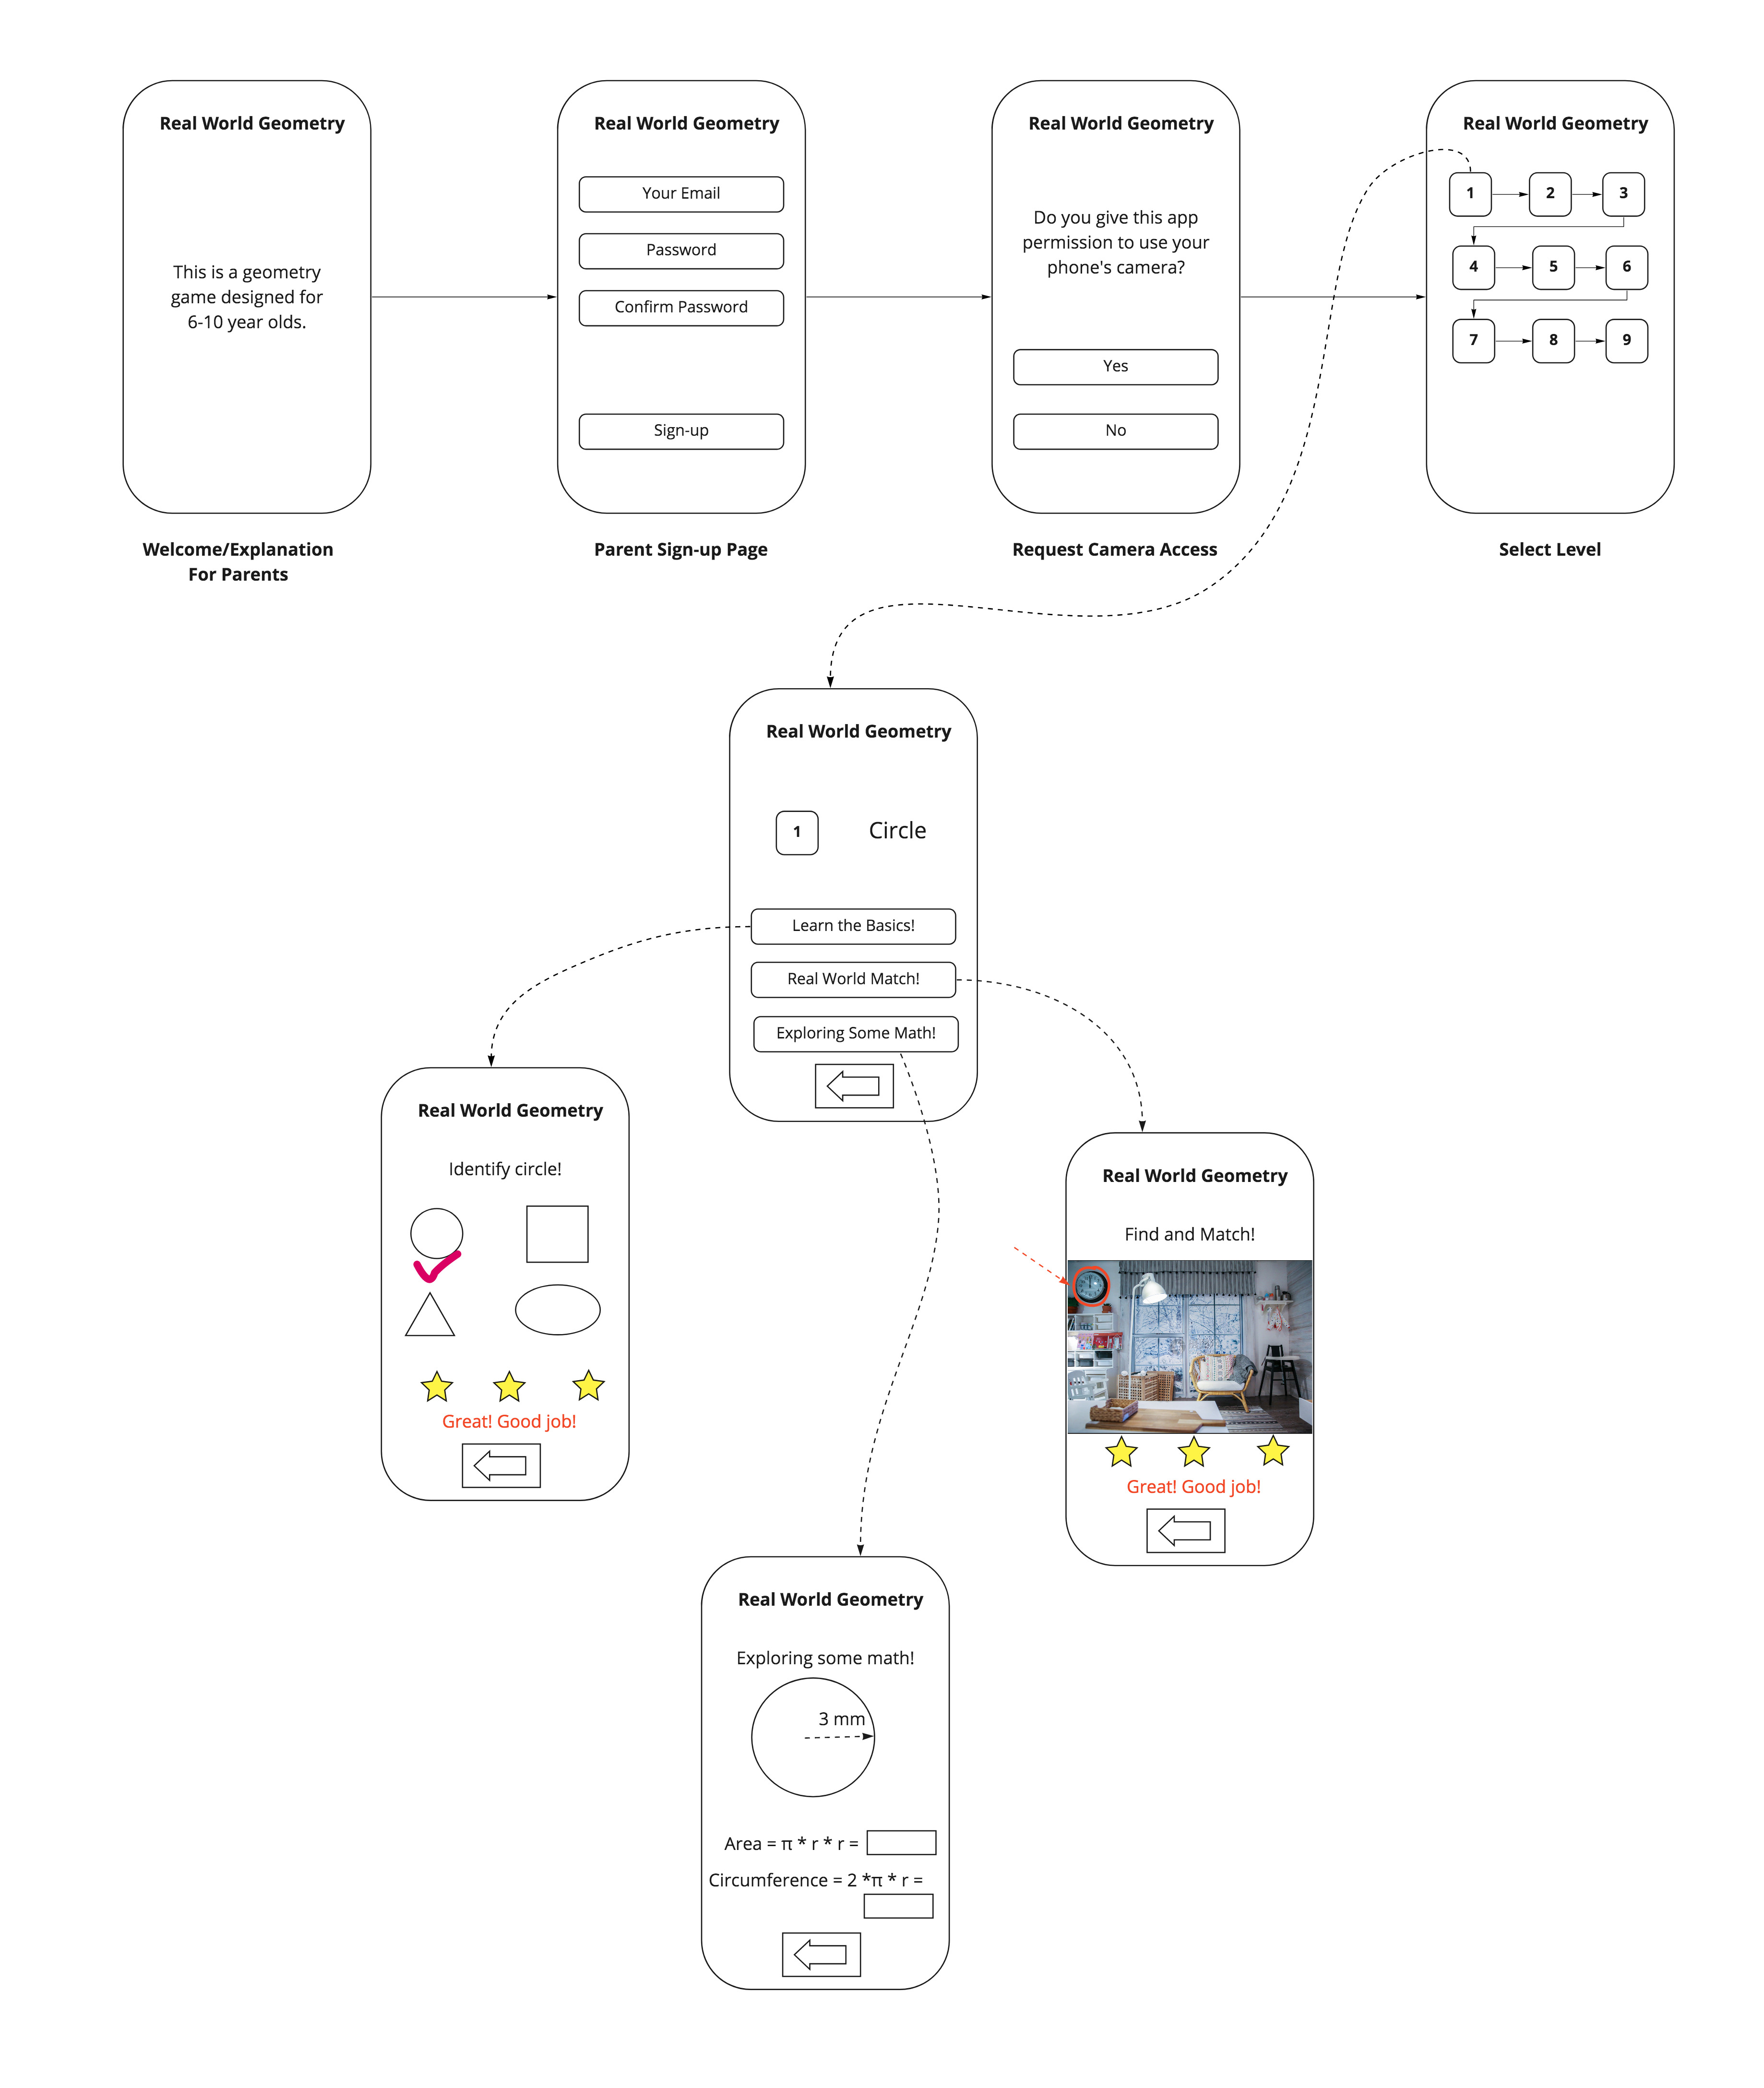
\includegraphics[width=\textwidth]{prototype.jpg}
  \newpage

  \section{User Study Questionnaire}
  \label{appendix:questionnaire}
  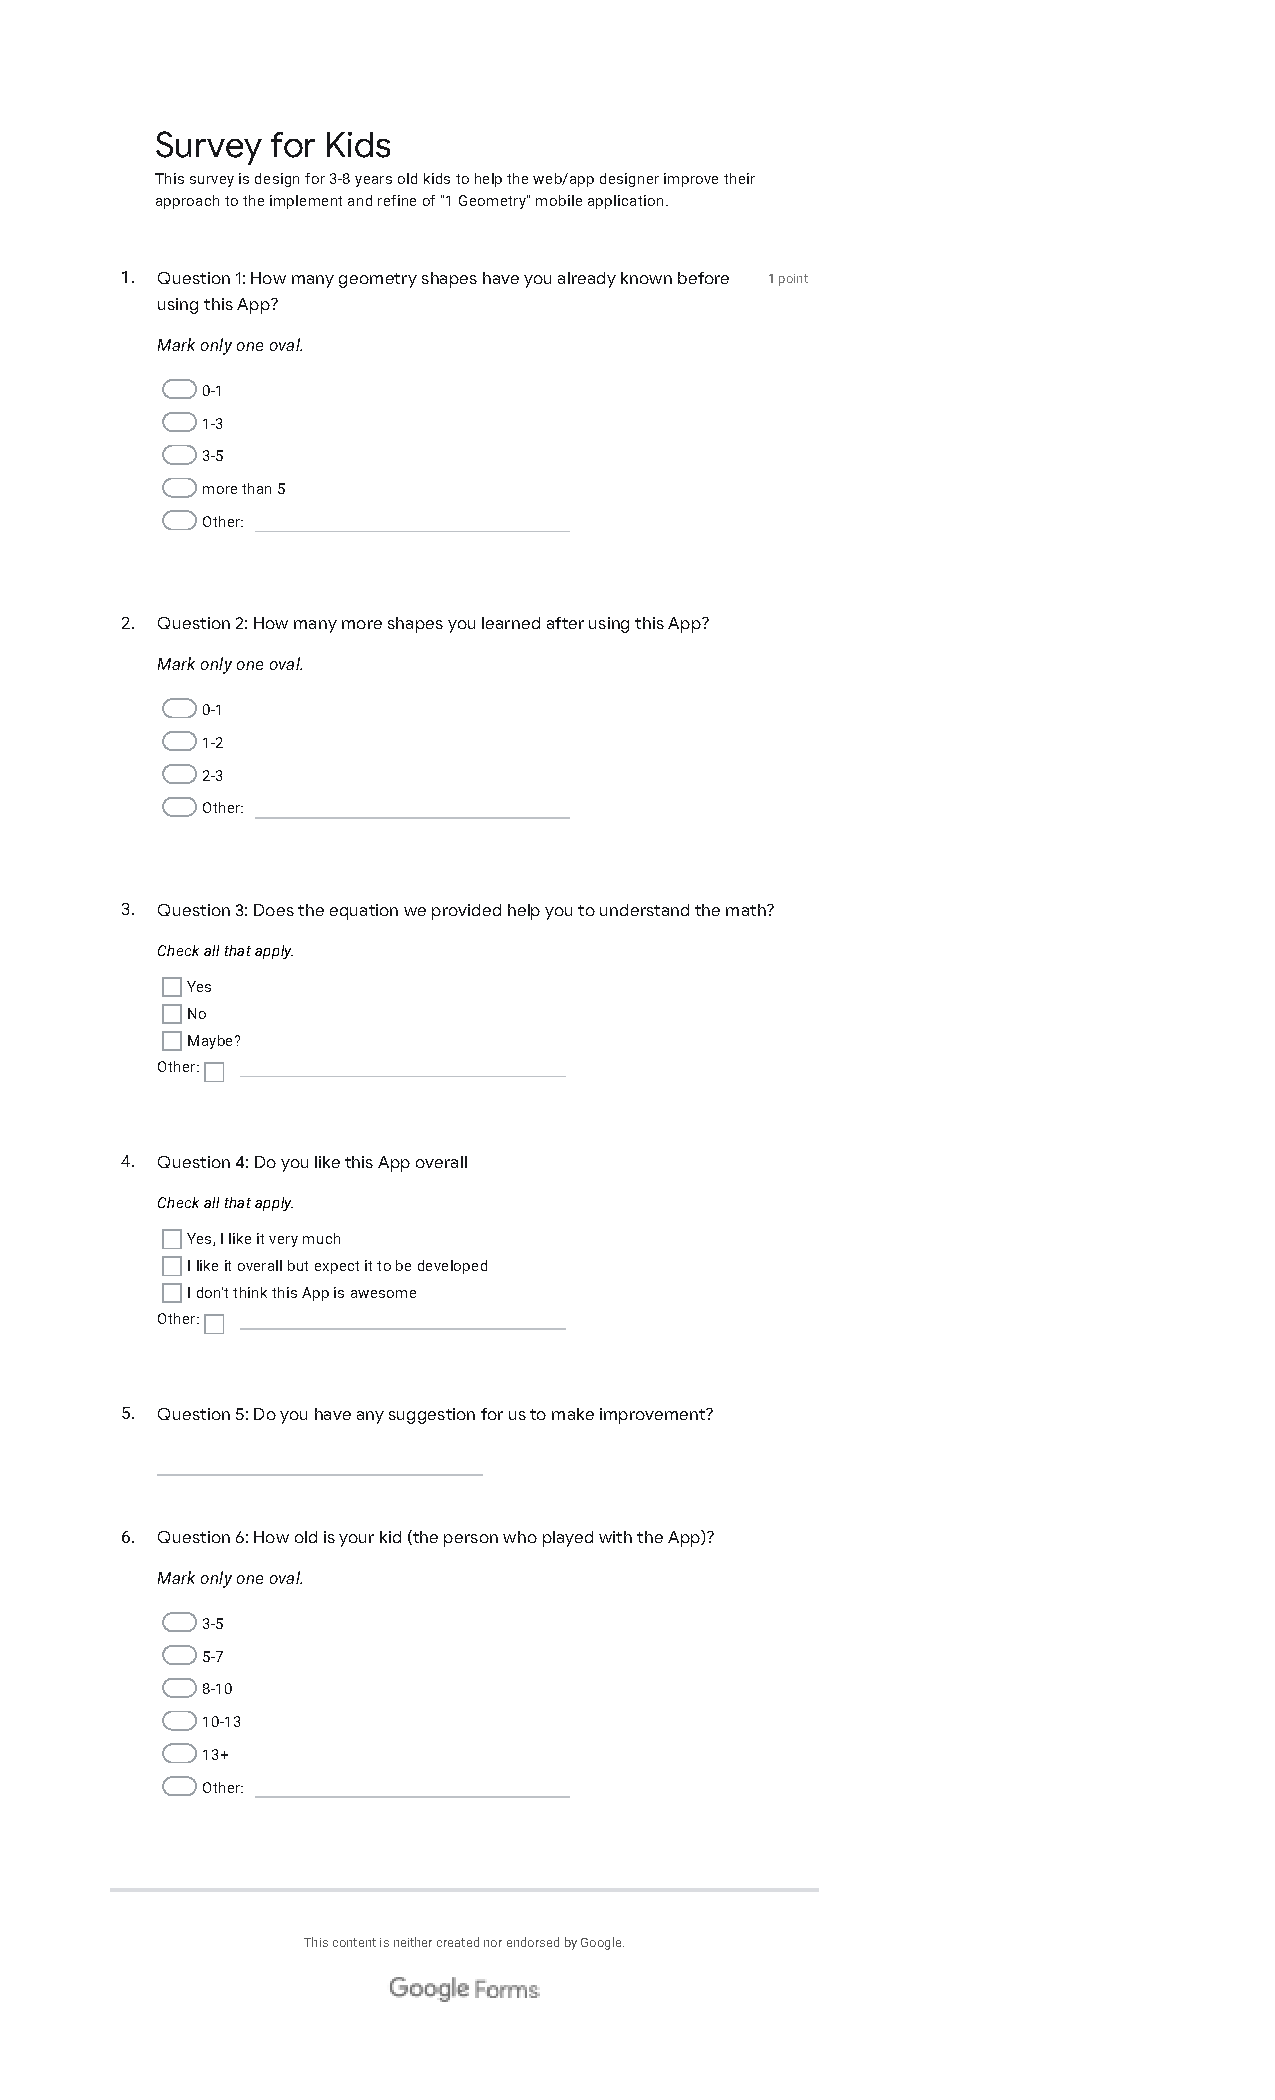
\includegraphics[width=\textwidth]{User-Study-Questionnaire.pdf}

\end{appendices}

\end{document}
